\documentclass{elsarticle}
\usepackage[utf8]{inputenc}
\usepackage[margin=2cm]{geometry}
\usepackage{graphicx}
\usepackage{multirow}
\usepackage{amssymb}
\usepackage{amsmath}
\usepackage{setspace}
\usepackage{outlines}
\usepackage{enumitem}
\usepackage{xcolor}
\usepackage{upgreek}
\usepackage{mathabx}
\usepackage{algorithm}
\usepackage{algorithmic}
\usepackage{amsthm}
\usepackage[labelfont=bf,font=small]{caption}
\usepackage{epsfig}
\usepackage{geometry}
\usepackage{subfigure}
\usepackage[textsize=tiny]{todonotes}
\usepackage[normalem]{ulem}
\usepackage{lipsum}
\usepackage{array}
\usepackage{booktabs}
\usepackage{lineno}
\usepackage{array}
\usepackage{tikz}
\usepackage[english]{babel}
\usepackage{animate}
\usepackage{cancel}

\usepackage[]{siunitx}
\sisetup{range-units=single,separate-uncertainty = true,print-unity-mantissa=false,per-mode=symbol,range-phrase = \text{--},
inter-unit-product=\cdot
}

\usepackage[
    protrusion=true,
    activate={true,nocompatibility},
    final,
    tracking=true,
    kerning=true,
    spacing=true,
    factor=1100]{microtype}
    
\SetTracking{encoding={*}, shape=sc}{40}

\usepackage{outlines}
\usepackage{enumitem}

\definecolor{lightblue}{rgb}{0.63, 0.74, 0.78}
\definecolor{seagreen}{rgb}{0.18, 0.42, 0.41}
\definecolor{orange}{rgb}{0.85, 0.55, 0.13}
\definecolor{silver}{rgb}{0.69, 0.67, 0.66}
\definecolor{rust}{rgb}{0.72, 0.26, 0.06}
\definecolor{purp}{RGB}{68, 14, 156}

\definecolor{zblue}{RGB}{8,81,156}
\definecolor{zpurp}{RGB}{84,39,143}
\definecolor{zred}{RGB}{165,15,21}

\colorlet{lightrust}{rust!50!white}
\colorlet{lightorange}{orange!25!white}
\colorlet{lightlightblue}{lightblue}
\colorlet{lightsilver}{silver!30!white}
\colorlet{darkorange}{orange!75!black}
\colorlet{darksilver}{silver!65!black}
\colorlet{darklightblue}{lightblue!65!black}
\colorlet{darkrust}{rust!85!black}
\colorlet{darkseagreen}{seagreen!85!black}



\usepackage{hyperref}
\hypersetup{
  colorlinks=true,
}
\usepackage{tabularx}
\usepackage{bbm}
\usepackage{bm}

\usepackage[nameinlink]{cleveref}
\crefname{equation}{}{}
\def\appendixname{}
\crefname{appendix}{}{}


\usepackage{setspace}
% \doublespacing
\setlength{\heavyrulewidth}{1.5pt}
% \setlength{\abovetopsep}{4pt}
 
\usepackage{soul}
\sethlcolor{yellow}

\usepackage[parfill]{parskip}

\usepackage{lineno}
\usepackage{tcolorbox}
%\linenumbers

\input{instr-mathsymbols}

\title{Your Paper}
\author{You}

\begin{document}
\begin{center}
    517 Mechanics of Soft Material HW2\\
    26311207 Wen-Ning, Wan
\end{center}
\section{Project II: Literature Review}
\subsection{Introductory context}
\begin{itemize}
    \item Shape memory polymers (SMPs) are materials that recover their original shape when stimulated by temperature \cite{xia2021review}. They typically exhibit two behaviors: processing, where the material is deformed and fixed into a temporary shape, and recovery, where it returns to its permanent shape upon heating \cite{lendlein2002shape}. These unique properties enable SMPs to be used in applications such as aerospace engineering \cite{liu2014shape} and biomedical devices \cite{zhang2014bioactive}. To fabricate SMPs, additive manufacturing is a widely used method, as it enables precise control over the original shape through CAD-guided design and production \cite{shen2024inverse}.
    \item Machine learning approaches are increasingly applied to materials science, where they can identify patterns in parameterized data and predict complex nonlinear behaviors \cite{chen2019machine, garces2021advances}. Machine learning has shown promise in modeling nonlinear responses \cite{liu2019deep} and can also facilitate inverse design, identifying material geometry to achieve specific target behaviors \cite{gu2018bioinspired}.

\end{itemize}

\subsection{The state of the field}
\begin{itemize}
    \item Neural network models are deployed as predictive models, where model parameters are optimized to minimize errors. Once the model is trained, these models can also be used in the inverse design process by systematically varying input parameters to identify configurations that yield target properties or behaviors \cite{park2024deep}.
    \item Experimental data for SMP honeycomb structures are typically obtained by submerging the samples in temperature-controlled water baths and applying mechanical loads via a load cell. This setup allows for the precise measurement of deformation during both programming and recovery phases while maintaining controlled temperature conditions \cite{ledari2025experimental}.
\end{itemize}

\subsection{The Big Gap}
Although additive manufacturing and uniaxial testing of SMP honeycomb structures have provided insight into their programming and recovery behaviors, no studies to date have demonstrated an inverse design approach for these systems. The major unknown is how structural geometry and manufacturing conditions together influence SMP behavior, which this work seeks to address.

\bibliographystyle{unsrt}
\bibliography{hw_ref} 

\section{Examples II: Kinetics, Constitutive Laws, and Viscoelasticity I}
\subsection{Balance of mass}
a)
Using the conservation of mass:
\begin{align*}
    &\rho_{,t}+\nabla_x\cdot(\rho v)=0\\
\end{align*}
Due to pure radial flow, divergence can be written as:
\begin{align*}
    &\nabla\cdot(\rho v)=\frac{1}{r^2}\frac{\partial}{\partial r}(r^2\rho v_r)\\
    \Rightarrow&\frac{\partial\rho}{\partial t}+\frac{1}{r^2}\frac{\partial}{\partial r}(r^2\rho v_r)=0\\
    \Rightarrow&\frac{\partial\rho}{\partial t}+\frac{1}{r^2}(2r\rho v_r+r^2\rho_{,r}v_r+r^2\rho v_{r,r})=0\\
    \Rightarrow&\rho_{,t}+\rho_{,r}v_r+\frac{\rho}{r}(2v_r+r v_{r,r})=0
\end{align*}
b)
Since it is assumed to be an incompressible flow, 
\begin{align*}
    \rho_{,t}=0
\end{align*}
The conservation of mass becomes:
\begin{align*}
    \frac{1}{r^2}\frac{\partial}{\partial r}(r^2\rho v_r)=0
\end{align*}
Since $\rho$ cannot be zero, the equation is deduced to:
\begin{align*}
    &\frac{\partial}{\partial r}(r^2 v_r)=0\\
    \Rightarrow&r^2v_r=C(t), \text{where C(t) is a function of t}
\end{align*}
At the wall of the bubble, 
\begin{align*}
    &\bm{v}(r,t) = \dot{R}\\
    \Rightarrow &C(t)=R^2\dot{R}=r^2v_r\\
    \Rightarrow &v_r=\frac{R^2\dot{R}}{r^2}
\end{align*}

\subsection{Balance of momenta}
a)\\
$F$ is the force acting on $\mathcal{B}$
\begin{align*}
    F&=\int_{\partial\Omega}tdS+\int_{\Omega}bdV\\
    &=-\rho_w g\int_{\partial\Omega}x_3\hat{n}dS-g\int_{\Omega}\rho(x)\bm{e_3}dV
\end{align*}
Using the divergence theorem:
\begin{align*}
    F&=-\rho_wgV\bm{e_3}+g\int_\Omega\rho\bm{e_3}dV\\
    &\int_{\Omega}\rho(x)dV=\frac{\frac{1}{2}\rho_w+\frac{3}{2}\rho_w}{2}V=\rho_wV\\
    F&=-\rho_w gV\bm{e_3}+g\rho_wV\bm{e_3}=0
\end{align*}
$M$ is the moment acting on $\mathcal{B}$
\begin{align*}
    M&=\int_{\partial\Omega}\bm{x}\times tdS+\int_{\Omega}\bm{x}\times bdV\\
    &=-\rho_w g\int_{\partial\Omega}\bm{x}\times(x_3\bm{\hat{n}})dS-g\int_{\Omega}\rho(x)\bm{x}\times\bm{e_3}dV\\
\end{align*}
Using the divergence theorem:
\begin{align*}
    &\int_{\partial\Omega}\bm{x}\times(x_3\hat{n})dS=\int_{\Omega}\bm{x}\times\nabla x_3 dV=\int_{\Omega}\bm{x}\times\bm{e_3}dV
\end{align*}
\begin{align*}
    M&=-g\int_{\Omega}(\rho_w+\rho(x))\bm{x}\times\bm{e_3}dV\\
    &=-g(-\bm{e_2}\int_{\Omega}(\rho_w+\rho(x))\bm{x}\times\bm{e_3}dV\\
    &=g\bm{e_2}B\int_{\Omega}x_1^2dV\\
    &=\frac{2\pi}{15}\rho_wgR^4e_2
\end{align*}
b)\\
If the net force $=0$, and the moment $=0$, $\mathcal{B}$ is static equilibrium. Since the fluid density is not uniform, $\mathcal{B}$ could be a static equilibrium.

\subsection{Viscoelastic data}
a)
The overall behavior of the material is not linear viscoelasticity, but if we consider the small deformation (eg. $\varepsilon < 0.1\%$ ), the material can be considered as linear viscoelasticity.\\
b)
$\sigma_0=100 \text{Pa}$
\begin{align*}
    \varepsilon(t)=J_c(t)\sigma_0
\end{align*}
Assume $J_c(t)=ae^{bt}+c$, by curve fitting, we get:
\begin{align*}
    J_c(t) = (-7.48\times10^{-3}e^{0.05t}+1.10\times10^{-2})\times100
\end{align*}
$\sigma_0=250 \text{Pa}$
\begin{align*}
    \varepsilon(t)=J_c(t)\sigma_0
\end{align*}
Assume $J_c(t)=ae^{bt}+c$, by curve fitting, we get:
\begin{align*}
    J_c(t) = (-1.00\times10^{-2}e^{-0.039t}+1.00\times10^{-2})\times250
\end{align*}
The fitting result of the two conditions is shown as follows:
\begin{figure}[h]
\centering
\begin{minipage}{0.45\textwidth}
\centering
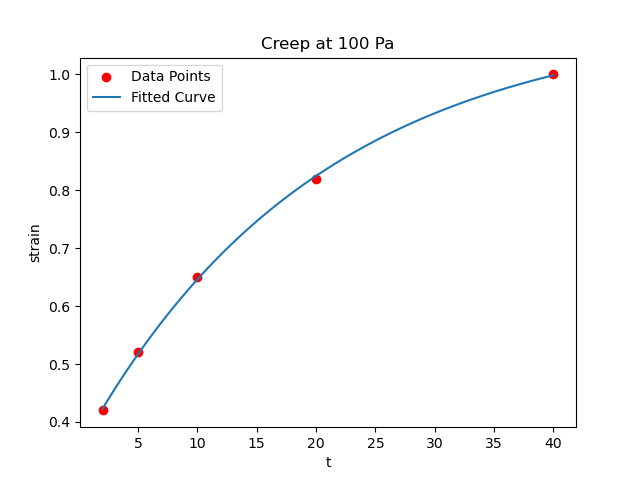
\includegraphics[width=\linewidth]{Hw_fig/1.png}
\label{fig:pic1}
\end{minipage}
\hfill
\begin{minipage}{0.45\textwidth}
\centering
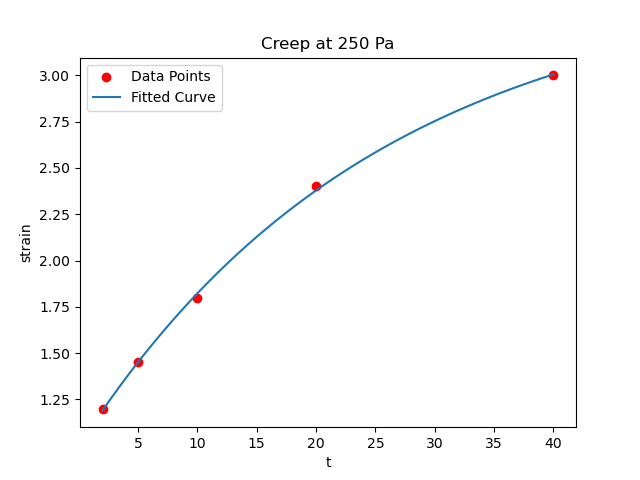
\includegraphics[width=\linewidth]{Hw_fig/2.png}
\label{fig:pic2}
\end{minipage}
\end{figure}

\subsection{Impulsive stresses}
a)\\
The general form of the creep relaxation function is:
\begin{align*}
    \varepsilon(t)&=J_c(t)\sigma_0+\int^t_0J_c(t-\tau)d\sigma(\tau)\\
    &=J_c(t)\sigma_0+\int^t_0J_c(t-\tau)A\delta(\tau)d\tau\\
    &=J_c(t)\sigma_0+A J_c(t)\\
    &=(A+\sigma_0)J_c(t)
\end{align*}
The Kelvin-Voigt solid model is:
\begin{align*}
    &\eta\dot{\varepsilon}+E\varepsilon=A\delta(t)\\
    &\eta(s\bar{\varepsilon}(s)-\varepsilon_0)+E\bar{\varepsilon}(s)=A\cdot 1\\
\end{align*}
Assume $\varepsilon_0 =0$
\begin{align*}
    &(\eta s+E)\bar{\varepsilon}(s)=A\\
    &\bar{\varepsilon}=\frac{A}{\eta s +E}=\frac{A}{\eta}\cdot\frac{1}{s+\frac{E}{\eta}}\\
    &\varepsilon(t)=\frac{A}{\eta}e^{\frac{-E}{\eta}t}
\end{align*}
b)\\
The general form of the creep relaxation function is:
\begin{align*}
    &\varphi(t)=\delta'(t)\\
    &\sigma(\tau)=B\delta'(t)\\
\end{align*}
\begin{align*}
    \varepsilon(t)&=J_c(t)\sigma_0+\int^t_0J_c(t-\tau)d\sigma(\tau)\\
    &=J_c(t)\sigma_0+\int^t_0J_c(t-\tau)B\delta'(\tau)d\tau\\
    &=J_c(t)\sigma_0+B\int^t_0J_c(t-\tau)\delta'(\tau)d\tau\\
    &=J_c(t)\sigma_0+BJ_c'(t)
\end{align*}
The Kelvin-Voigt solid model is:
\begin{align*}
    &\eta\dot{\varepsilon}+E\varepsilon=B\varphi(t)\\
    \Rightarrow&\eta\dot{\varepsilon}+E\varepsilon=B\delta'(t)\\
    &\eta(s\bar{\varepsilon}(s)-\varepsilon_0)+E\bar{\varepsilon}(s)=B\cdot s\\
\end{align*}
Assume $\varepsilon_0 =0$
\begin{align*}
    &(\eta s+E)\bar{\varepsilon}(s)=B\cdot s\\
    &\bar{\varepsilon}=\frac{Bs}{\eta s +E}=\frac{B}{\eta}\cdot(\frac{s+\frac{E}{\eta}}{s+\frac{E}{\eta}}-\frac{\frac{E}{\eta}}{s+\frac{E}{\eta}})\\
    &\varepsilon(t)=\frac{B}{\eta}(\delta (t)-e^{\frac{-E}{\eta}t})
\end{align*}
\subsection{Two-element models}
a)\\
The displacement on the top plate is:
\begin{align*}
    x(t) = d(1-cos(\omega t))
\end{align*}
The strain function can be denoted as:
\begin{align*}
    \varepsilon(t)=\frac{d}{h}(1-cos(\omega t))
\end{align*}
Applying to the Kelvin-Voigt model
\begin{align*}
    &\eta \dot{\varepsilon}+E\varepsilon=\sigma\\
    &\sigma(t) = \omega \eta \frac{d}{h}(sin(\omega t))+E\frac{d}{h}(1-cos(\omega t))
\end{align*}
b)\\
Consider the periodic terms:
\begin{align*}
    &\varepsilon(t)=\frac{-d}{h}cos(\omega t)\\
    &\sigma (t)=\omega \eta\frac{d}{h}sin(\omega t)-E\frac{d}{h}cos(\omega t)
\end{align*}
Make the functions into the form of $sin(wt+\alpha)$
\begin{align*}
    \varepsilon(t)=\frac{d}{h}sin(\omega t  -\frac{\pi}{2})
\end{align*}
Let $\alpha_1=-\frac{\pi}{2}$
\begin{align*}
    &\sigma (t)=\sqrt{(\omega \eta\frac{d}{h})^2+(-E\frac{d}{h})^2}sin(\omega t+\alpha_2)\\
    &tan(\alpha_2)=\frac{-E}{\omega\eta}\\
    &\delta=\alpha_2-\alpha_1=arctan(\frac{-E}{\omega\eta})+\frac{\pi}{2}\\
    &tan\delta=\frac{\omega\eta}{E}
\end{align*}
c)\\
\begin{align*}
    &\eta\dot{\varepsilon}+E\varepsilon=-\sigma_0-\sigma_0 sin(\omega t)\\
    &\eta(s\bar{\varepsilon}(s)-\varepsilon(0))+E\bar{\varepsilon}(s)=-\frac{\sigma_0}{s}-\sigma_0\frac{w}{s^2+w^2}\\
    &(\eta s+E)\bar{\varepsilon}(s)=-\frac{\sigma_0}{s}-\frac{\sigma_0 w}{s^2+w^2}\\
    &\bar{\varepsilon}(s)=-\frac{\sigma_0}{s(\eta s+E)}-\frac{\sigma_0\omega}{(s^2+w^2)(\eta s+E)}\\
    \Rightarrow&\varepsilon(t)=-\frac{\sigma_0}{\eta}(1+e^{\frac{-Et}{\eta}})+\frac{\sigma_0\omega\eta}{E^2+\eta^2\omega^2}cos(\omega t)-\frac{\sigma_0 E}{E^2+\eta^2\omega^2}sin(\omega t)-\frac{\sigma_0}{\eta}e^\frac{-Et}{\eta}
\end{align*}
Consider the periodic terms:
\begin{align*}
    &\varepsilon=\frac{\sigma_0\omega\eta}{E^2+\eta^2\omega^2}cos(\omega t)-\frac{\sigma_0 E}{E^2+\eta^2\omega^2}sin(\omega t)\\
    &\sigma (t)=-\sigma_0 sin(\omega t)\\
    &\alpha_1=arctan(\frac{\omega\eta}{-E})\\
    &\alpha_2=\pi\\
    &\delta=\alpha_1-\alpha_2=arctan(\frac{\omega\eta}{-E})-\pi\\
    &tan\delta=-\frac{\omega\eta}{E}
\end{align*}
d)\\
$tan\delta_1=\frac{\omega\eta}{E}$ and $tan\delta_1=-\frac{\omega\eta}{E}$. Take the absolute value of two conditions, $|tan\delta_1|=|tan\delta_2|$
\end{document}